\section{Chords}

\subsection{Building chords}
In the previous sections we have learned about the major and minor scales. This information can be used to finally start to learn about chords.

\textbf{A major or minor chord is constructed by playing the 1st, 3rd and 5th note of a scale at the same time. That's it.}

\subsection{Open and barre chords}

When a chords is played that contains open strings, it is called an "open chord". When a chord is played without open strings, it is called a "barre chord".

The nice thing about barre chords is that you can move them up and down the neck. At that point the barre chord becomes more of a shape than a chord per se. Depending on what the root note is at a certain position, the barre chord will get a different name. We will see this later in the \textbf{CAGED system}.

On the next page in \autoref{fig:guitar_major_minor_chords} you will see all the major and minor chords listed. The chord \textbf{C} is a major chord and the chord \textbf{Cm} is a minor chords. The same holds for the other chords. Below each chords there are the 1st, 3rd and 5th notes from the respective scale (see \autoref{tab:guitar_natural_note_major_scale} and \autoref{tab:guitar_natural_note_minor_scale}).

The green dots indicate the root note. This is the note with the same name as the chord.

A couple things to note:

\begin{itemize}
	\item The root and the 5th note of a scale are same for both the major and minor variant.
	\item The 3rd note of minor chord is always a half step / 1 semitone lower than it is in the major chord.
\end{itemize}

The barre F chord is a good example of what was mentioned in the beginning. The thing about barre chords to become more like a shape that can become different chords. Compare the shape of the E and Em chords with the F and Fm chord shapes. Note how the shape is the same and there are no open strings in the F and Fm. By just moving the E chord shape a half step (one fret) to the right, the root note has changed and it is therefore now an F chord.

\newpage

\begin{figure}[h]
	\centering
	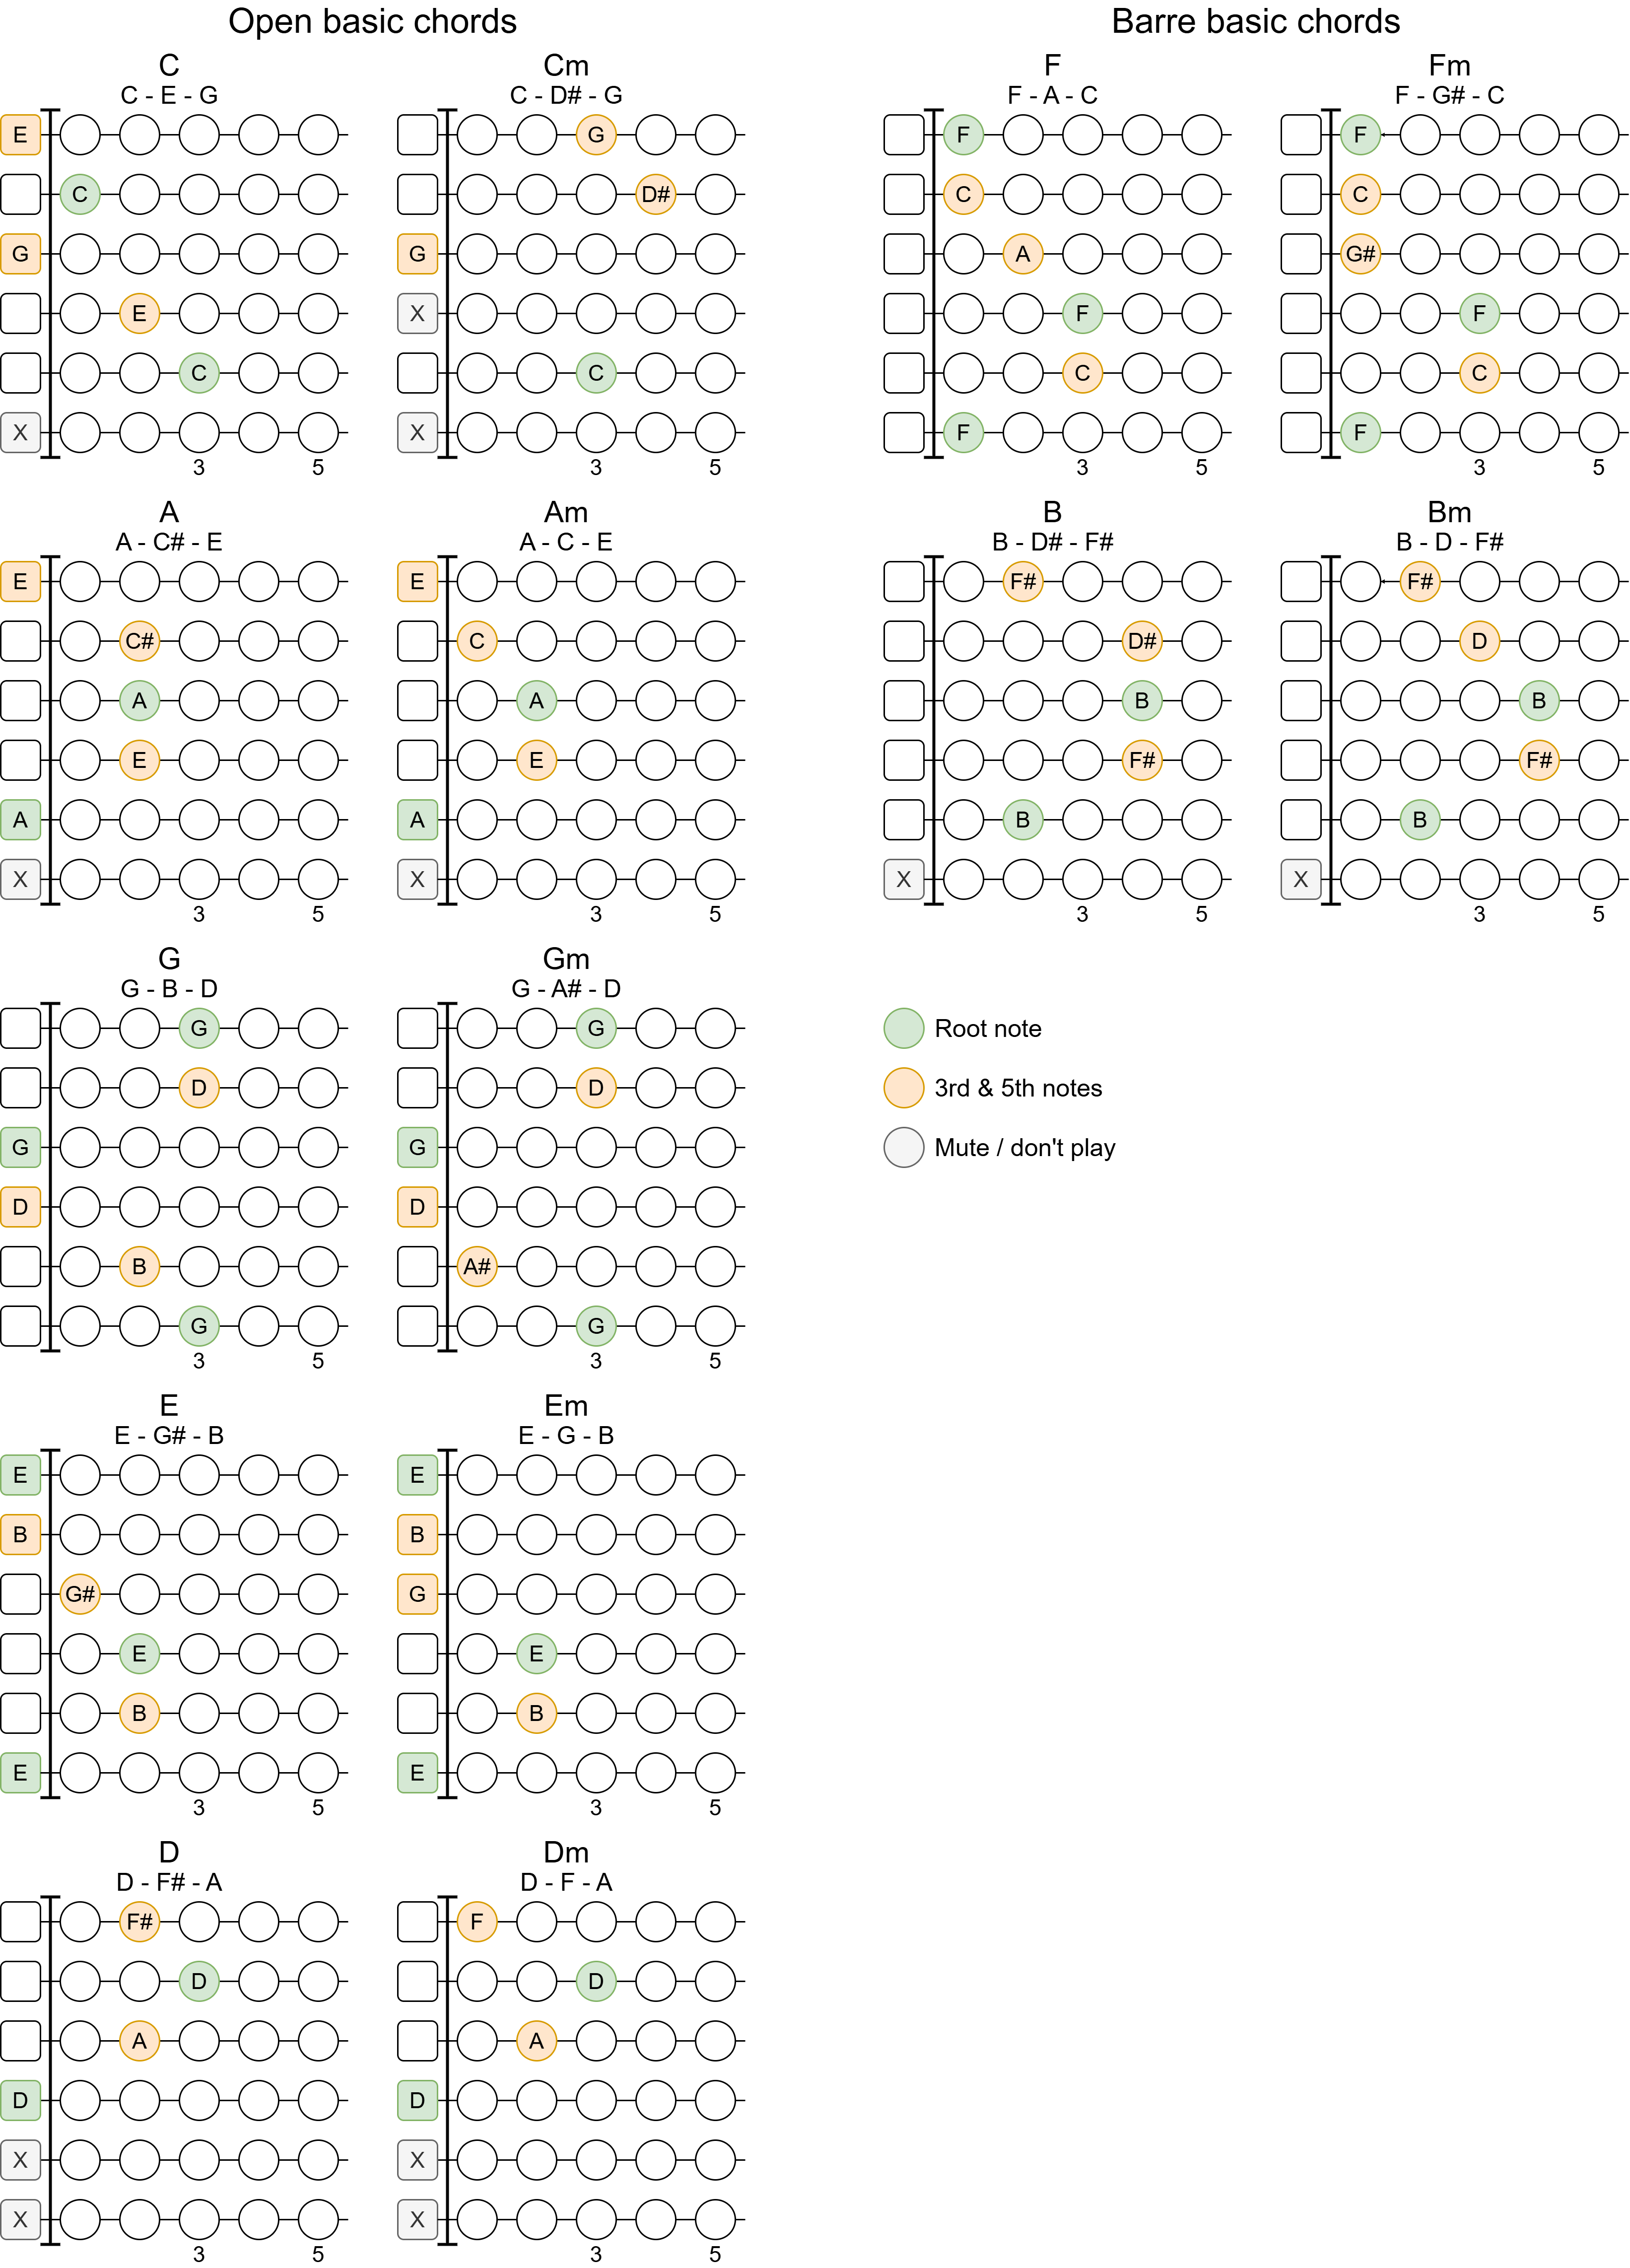
\includegraphics[height=0.9\textheight]{../../Images/GuitarBasicChords.png}
	\caption{Major and minor chords}
	\label{fig:guitar_major_minor_chords}
\end{figure}

\clearpage

Lets play some chords. The theme song (\autoref{fig:guitar_adventure_time}) of the Adventure Time series is a good start. The notes on the staff here are replaced by rhythm notation. The duration of the note shapes is still the same. But now it only indicates the strumming rhythm.

\begin{figure}[h]
	\centering
	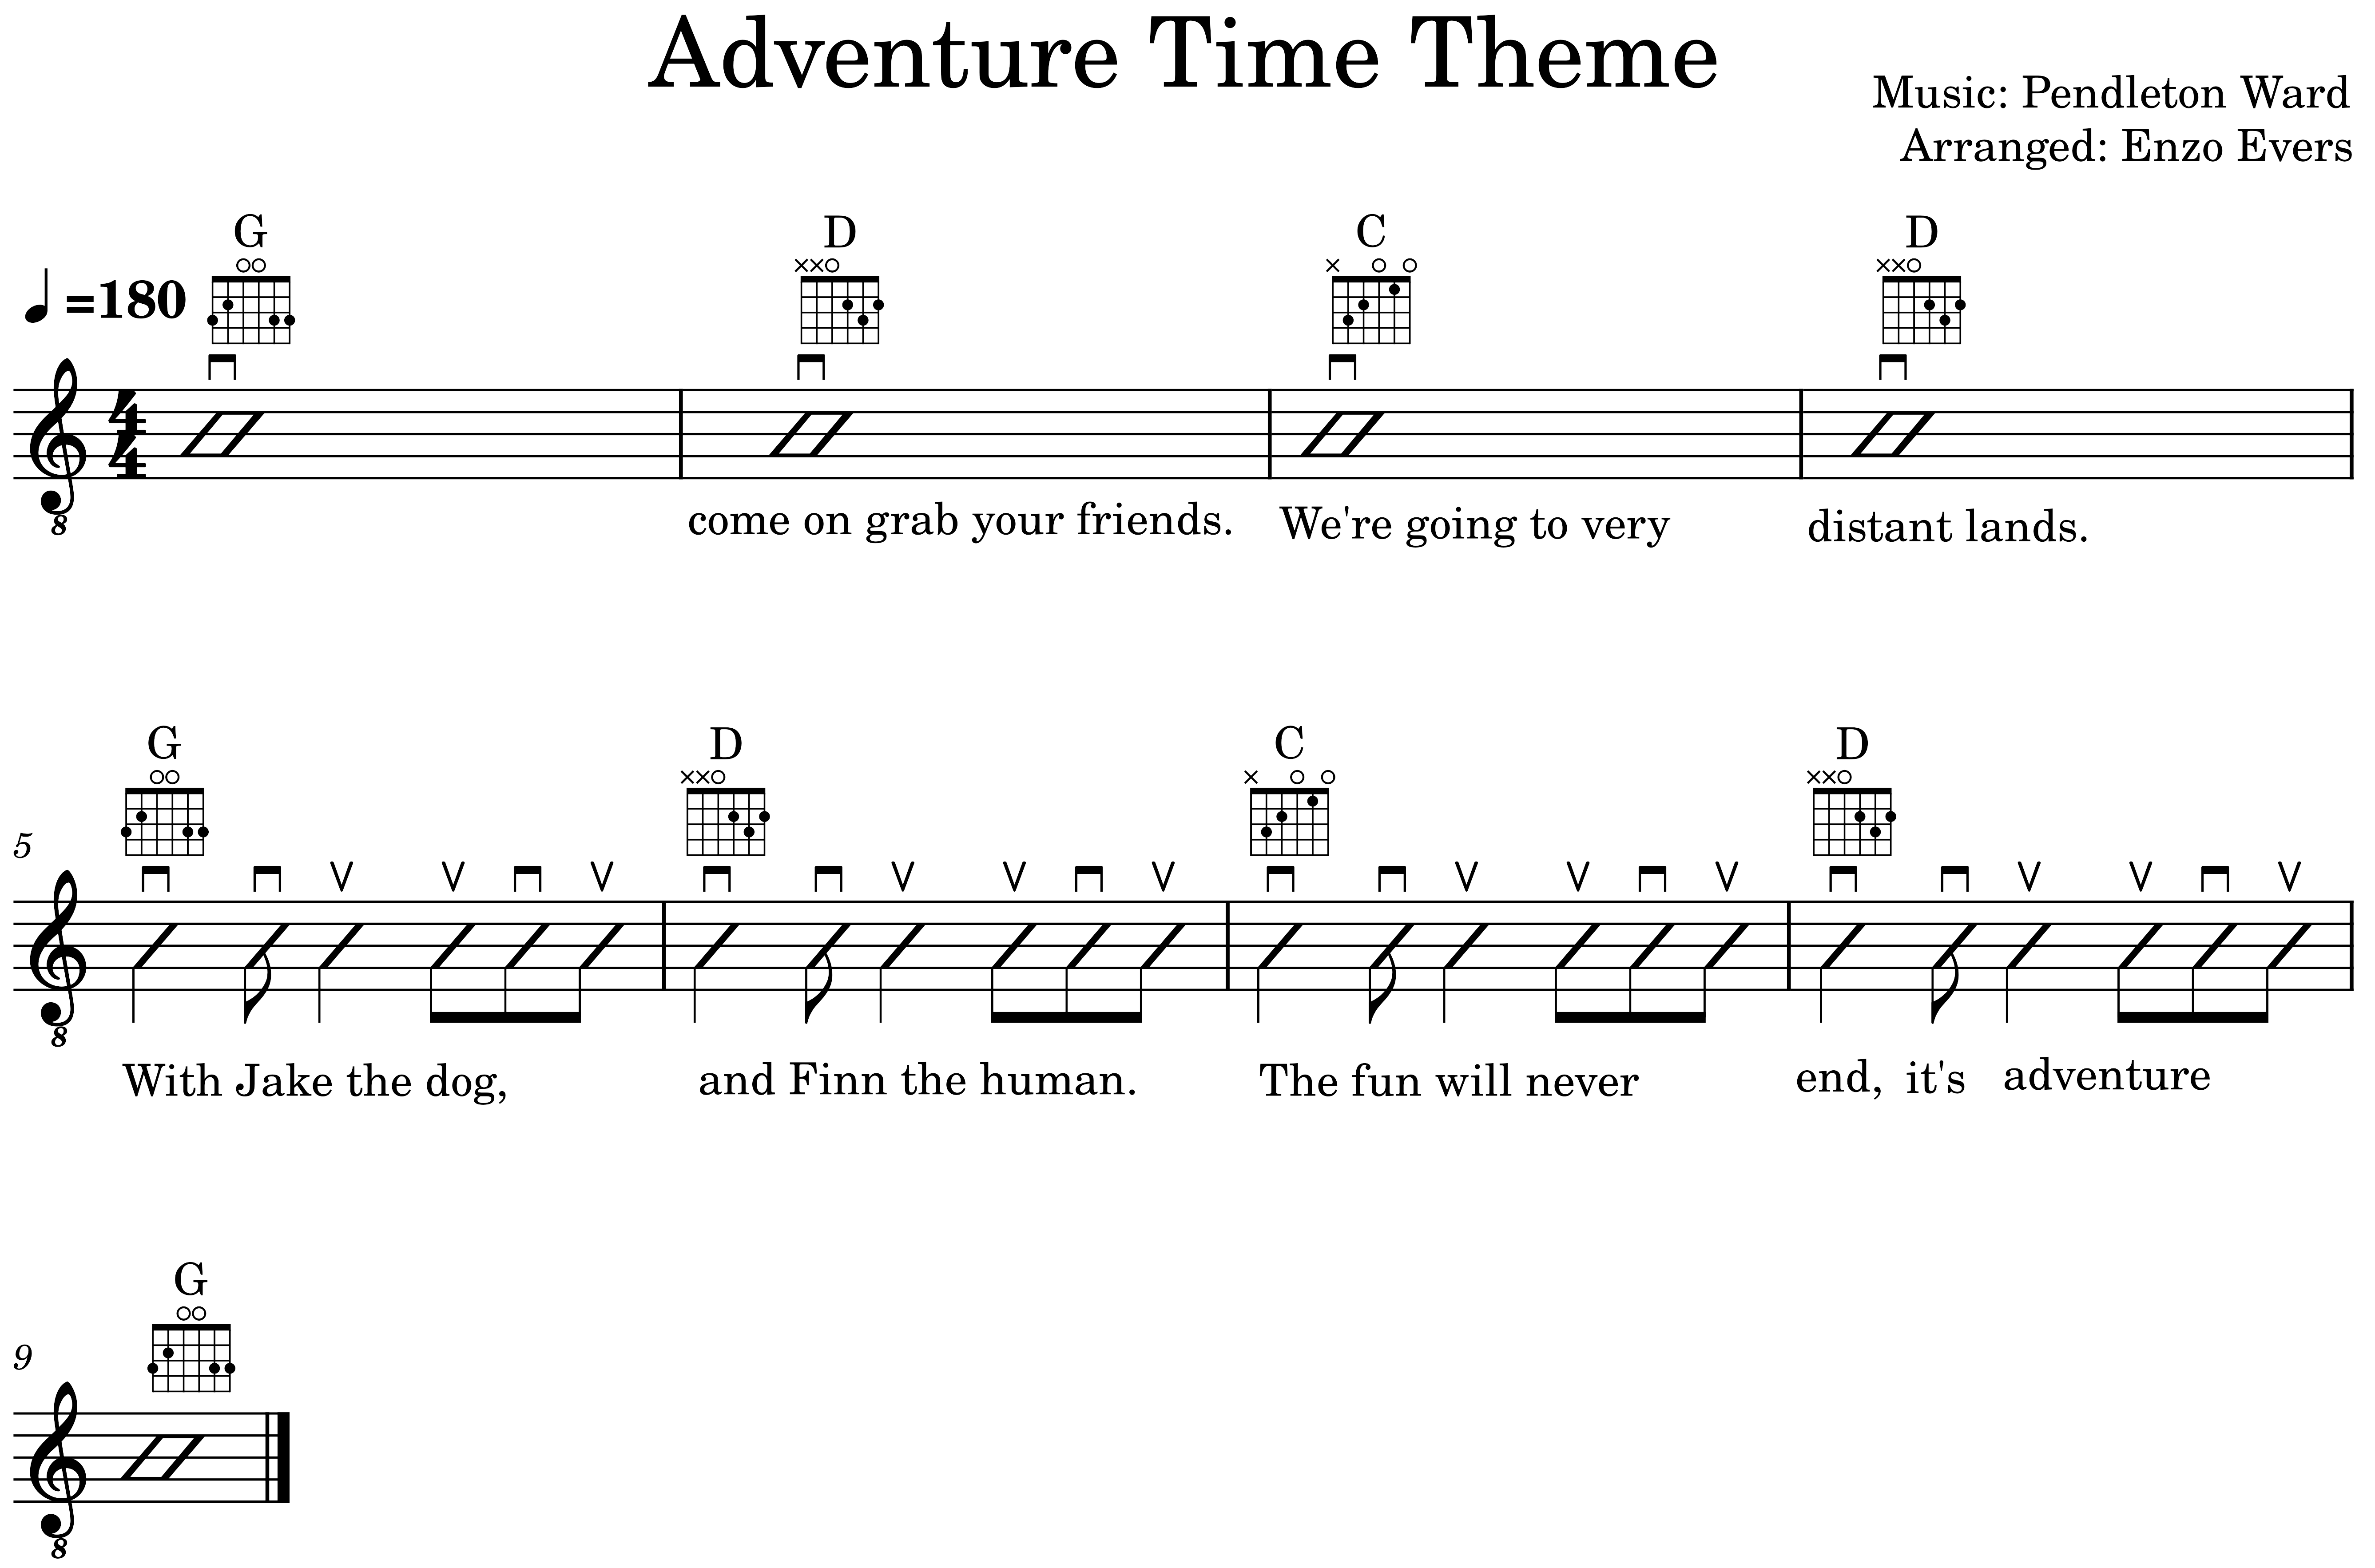
\includegraphics[width=\textwidth]{../../MuseScore/Guitar/GuitarAdventureTimeTheme.png}
	\caption{Adventure Time Theme Song}
	\label{fig:guitar_adventure_time}
\end{figure}

\newpage

In the song "Knockin' On Heaven's Door" By Bob Dylan, the same chords are used as in the Adventure Time theme, plus one extra chord. The \textbf{Am}.

\begin{song}[verse/numbered, remember-chords, align-chords=l]{title={Knockin' On Heaven's Door - Bob Dylan}, music={Bob Dylan}}
	\begin{intro}	
		^{G}   ^{D}      ^{Am}     ^{G}Oo ^{D}oo-oo ^{C}oo \\
		^{G}Oo ^{D}oo-oo ^{Am}oo   ^{G}Oo ^{D}oo-oo ^{C}oo \\
	\end{intro}
	\begin{verse}
		^{G}Mama, take this ^{D}badge off of me ^{Am} \\
		^{G}I can’t ^{D}use it anymore ^{C} \\
		^{G}It’s gettin’ ^{D}dark, too dark for me to see ^{Am} \\
		^{G}I feel like I’m ^{D}knockin’ on heaven’s door ^{C} \\
	\end{verse}
	\begin{chorus}
		^{G}Knock, knock, ^{D}knockin’ on heaven’s ^{Am}door \\
		^{G}Knock, knock, ^{D}knockin’ on heaven’s ^{C}door \\
		^{G}Knock, knock, ^{D}knockin’ on heaven’s ^{Am}door \\
		^{G}Knock, knock, ^{D}knockin’ on heaven’s ^{C}door \\
	\end{chorus}
	\begin{verse}
		^Mama, put my ^guns in the ground ^ {} \\
		^I can’t ^shoot them anymore ^ {} \\
		^That long black ^cloud is comin’ down ^ {} \\
		^I feel like I’m ^knockin’ on heaven’s door ^ {} \\
	\end{verse}
	\begin{chorus}
		^Knock, knock, ^knockin’ on heaven’s ^door \\
		^Knock, knock, ^knockin’ on heaven’s ^door \\
		^Knock, knock, ^knockin’ on heaven’s ^door \\
		^Knock, knock, ^knockin’ on heaven’s ^door \\
	\end{chorus}
\end{song}

\newpage

Another song to practice chord changes with with can be "Hey Ya!" from Outkast. This only uses four chords, and the order of the chords is the same throughout the whole song.

To give a feeling for the chords, the first part of the song is shown here. You can listen to the song and play these chords for the rest of the song.

\begin{song}[verse/numbered, align-chords=l]{title={Hey Ya! - Outkast}, music={Outkast}}
	\begin{intro}
		One, two, three, uh!
	\end{intro}
	\begin{verse}
		^{G}My baby don't ^{C}mess around \\
		Because she loves me so, and this ^{D}I know for ^{E}sure (Uh) \\
		^{G}But does she ^{C}really wanna \\
		But can't stand to see me walk ^{D}out the ^{E}door? (Ah) \\
	\end{verse}
\end{song}

There are two (actually 4) more important shapes to learn. The barre shapes. These are shown in \autoref{fig:guitar_major_minor_chords} as the F and B chords. For these chords you place your index finger over all the strings, and use the remaining fingers to press the remaining notes. Note that for the B chord you only have to place your index finger over the first 5 strings. \autoref{fig:guitar_barre_hand_shape_f} show how to play the F-shape barre chord. For the B-shape the hand position is similar.


\begin{figure}[h]
	\centering
	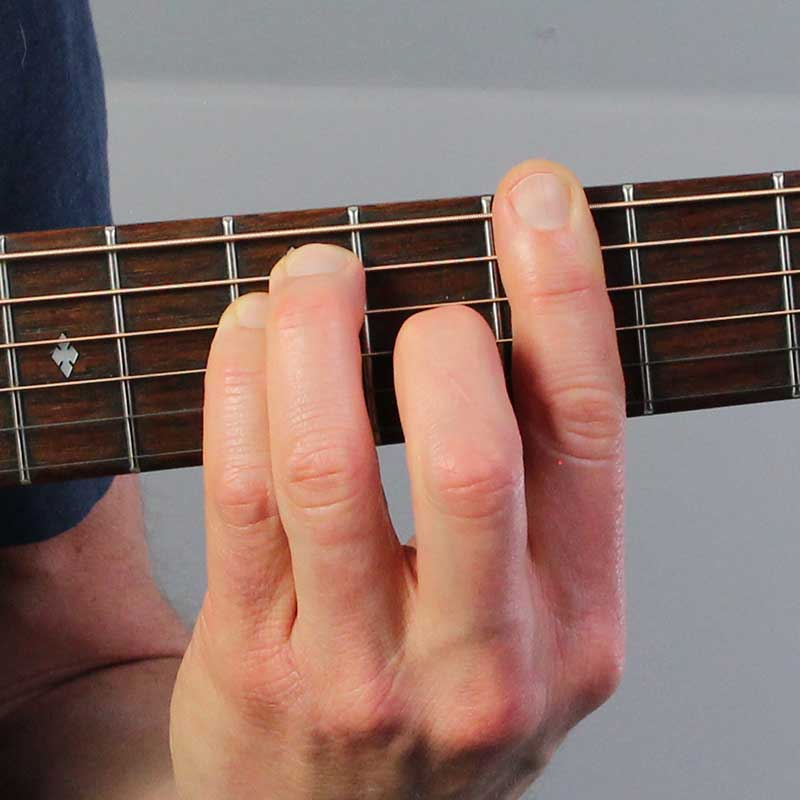
\includegraphics[width=0.5\textwidth]{../../Images/Barre-E-shape-fingers-added.jpg}
	\caption{Hand position for a barre chord with the F shape \cite{BarreHandPositionGuitar}}
	\label{fig:guitar_barre_hand_shape_f}
\end{figure}

\newpage

The song "Perfect" by Ed Sheeran is a good song to practice both shapes. This also shows the power of barre chords. The facts that they can be moved up and down the neck to make different chords.

The song uses 4 chords: A$\flat$, Fm, D$\flat$, and E$\flat$.

While some of these chords could be played as an open chord, it's not the most comfortable. We could use a capo to make it easier. But that would take away a good learning opportunity. But more seriously, maybe you don't have a capo at your disposal when you want to play this song. So it's still good to learn how to use these barre chords.

Only the first verse is shown here to focus on the barre chords themselves. The barre chords to use are shown in \autoref{fig:guitar_barre_chords_perfect_ed_sheeran}. Note the numbers below the shapes. These are the fret numbers.


\begin{figure}[h]
	\centering
	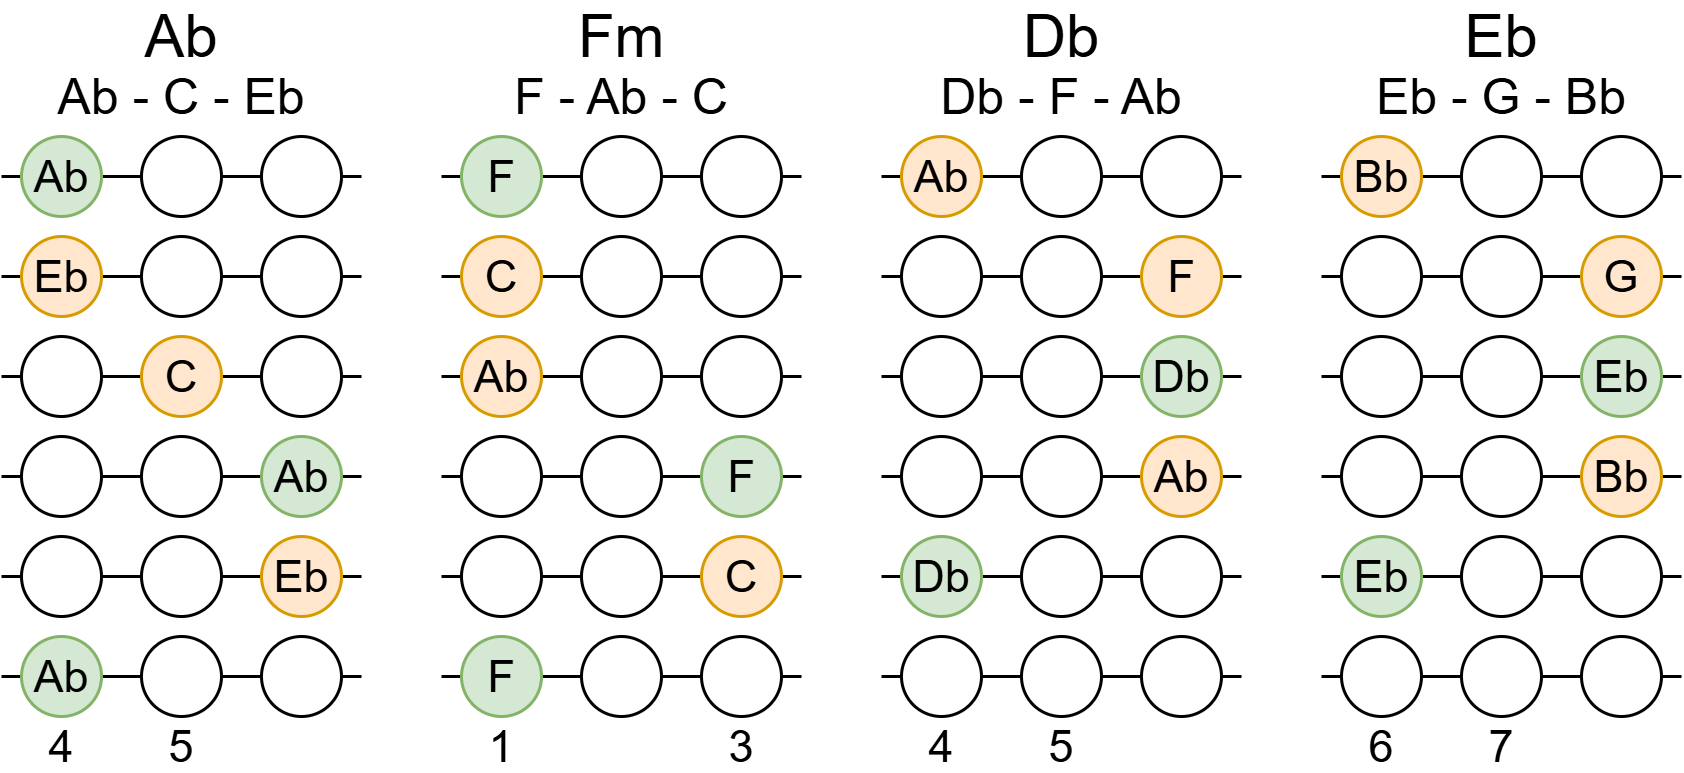
\includegraphics[width=0.8\textwidth]{../../Images/ChordsUsedInPerfectEdSheeran.png}
	\caption{Barre chords used in "Perfect - Ed Sheeran"}
	\label{fig:guitar_barre_chords_perfect_ed_sheeran}
\end{figure}


Note how the shapes are all very similar, but that note of the lowest root note indicates which chord it is.

\begin{song}[verse/numbered, align-chords=l]{title={Perfect - Ed Sheeran}, music={Ed Sheeran}}
	\begin{verse}
		I found a ^{Ab}love for ^{Fm}me \\
		Oh, darling, just ^{Db}dive right in and follow my ^{Eb}lead \\
		Well, I found a ^{Ab}girl, beauti^{Fm}ful and sweet \\
		Oh, I never ^{Db}knew you were the someone waitin' for^{Eb}me \\
	\end{verse}
\end{song}

\subsection{Your turn}

We've played all kind of different chords now. It's up to you to see which song you want to play, look up the chords on the internet, and practice the chord transitions. Feel free to play the chords in different ways (open chord, F(m)-shape, B(m)-shape, etc.). Each option gives a different sound, or maybe one option is easier to play than another. Just experiment!